\chapter{Analysis and Design}

\section{Introduction}
Introduce what this chapter is going to present.

\section{OAuth}
In each of our service provider implementation that supported it, we made use of OAuth2 for authorization.  OAuth is a widely used authorization protocol which allows resource owners (typically users) to authorize third-party applications, granting them access to protected (access-restricted) resources, while promoting user security and developer simplicity.  

Traditionally, to access restricted resources hosted on the server, a client application uses the user's own credentials  to make the request. This means that the user is required to share their private credentials with the application, which is a source of many issues and limitations. One example is that the third-party clients need to store credentials, typically in vulnerable plain-text form,  in order to use them again in the future. If the application is then compromised at any point, the attacker can easily access the stored user credentials and any resources they protect. Another disadvantage is that with the direct use of credentials, users cannot limit what applications can access and for how long, and revoking access to a third party also revokes access to all other parties, since the password needs to be changed. Finally, this scheme requires resource servers themselves to have authentication capabilities ~\cite{oauth}.

OAuth resolves these problems by not relying on user credentials to gain access to protected resources, but instead by having the client obtain a string, called an access token, from an authorization server (might be the resource server or another server).  The token can also specify various attributes like access scope and duration. As a result, an additional authorization layer is added, while the client is decoupled from the resource owner, since the latter's credentials need not be shared. The OAuth flow, which is depicted in figure \ref{fig:oauth_flow}, can be summarized as follows ~\cite{oauth}:

\begin{enumerate} [(A.)]
	\item The client makes an authorization request to either the resource owner  (as shown) or, preferably, to the intermediary authorization server. 
	
	\item The resource owner returns an authorization grant, a credential which represents their authorization, using one of the grant types that are discussed later in this section. 
	
	\item The client authenticates with the authorization server and presents the grant, in order to request an access token.
	
	\item An access token is issued to the client, if validation of the authorization grant is successful. Additionally, an optional refresh token can also be returned here, which allows the client to later obtain a new access token when the previous one is invalidated or expires.
	
	\item  The client authenticates with the resource server by presenting the token and requests a restricted resource.
	
	\item If the access token is valid, the resource server returns the requested resource.
\end{enumerate}

\begin{figure} [h]
	\centering
	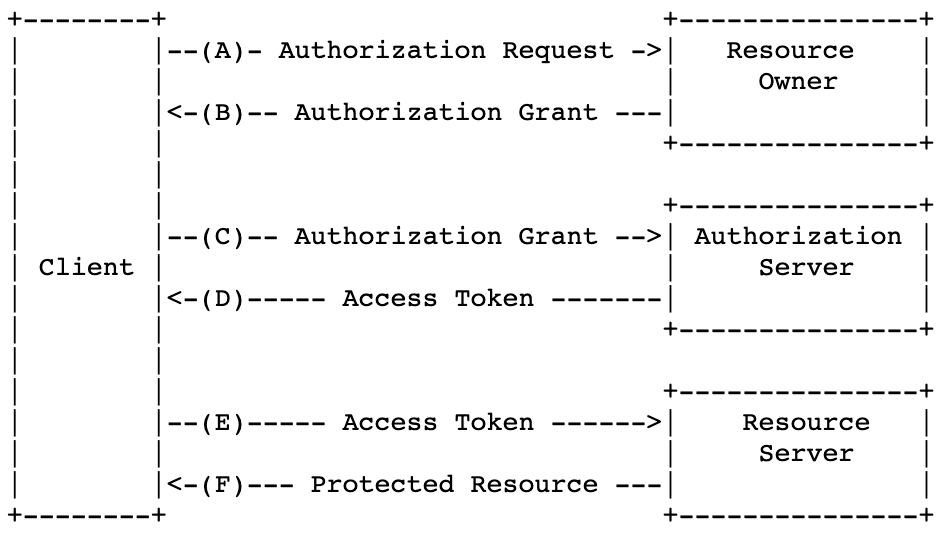
\includegraphics[scale=0.7]{images/oauth_flow}
	\caption{\label{fig:oauth_flow}Abstract OAuth Flow}
\end{figure}

The available OAuth grant types are ~\cite{oauth, oauth_grants}:

\begin{itemize}
	\item [--]The \textit{Authorization Code} grant type involves an intermediary authorization server to which the user is first redirected by the client. Then, the authentication server authenticates the user and obtains authorization. This is the preferred grant type, as the user's credentials aren't shared with the client and the access token is directly transmitted to the client, minimizing exposure. 
	
	\item [--] The \textit{\ac{pkce}} extends the Authorization Code grant type, by making the client use a secret when exchanging the authorization code, after creating it during the authorization request. Because the token request now depends on the secret, intercepting the authorization code is not harmful and so, PCKE helps prevent code injection attacks and \ac{csrf}.
	
	\item [--] \textit{Client Credentials} can be used as an authorization grant usually when the access scope is limited to the client's own resources. 
	
	\item [--] The \textit{Device Authorization Grant} is especially applicable when devices that don't have convenient input capability or a web browser are involved. Example devices include Apple TVs and printers. These devices instruct the user to visit a particular web-page on another device so that authorization can be completed. While the user is busy with the authorization flow, the original device starts requesting the access from a specific endpoint.
\end{itemize}

For our implementation, only 2 cloud provider \ac{sdk}s didn't directly integrate with OAuth2 for authentication, namely Amazon's Boto3 and Microsoft Azure's SDK.

\section{Summary}
